% -------------------------------------- PARTE II -------------------------------------


\newpage
\section*{\hfil Parte II\hfil}

\section{Questões e Respostas}

\subsection{Questão 1 - Topologia LEI-RC}
\subsubsection{Indique que endereços IP e máscaras de rede foram atribuídos pelo CORE a cada equipamento. Para simplificar, pode incluir uma imagem que ilustre de forma clara a topologia definida e o endereçamento usado.}

    Pela Figura \ref{parteII-questao1-topologia} conseguimos ter uma visão geral da topologia assim como a divisão entre os vários departamentos. Assim, a todos os endereços é aplicada uma máscara de rede de 25  \textit{bits}, sendo os endereços das sub-redes dos departamentos os seguintes: 

    \begin{multicols}{2}
    \begin{itemize}
        \item \textbf{Departamento A:} 10.0.4.0 
        \item \textbf{Departamento B:} 10.0.5.0 
        \item \textbf{Departamento C:} 10.0.6.0 
        \item \textbf{Departamento D:} 10.0.7.0 
    \end{itemize}
    \end{multicols}


    \begin{figure}[H]
    \centering
    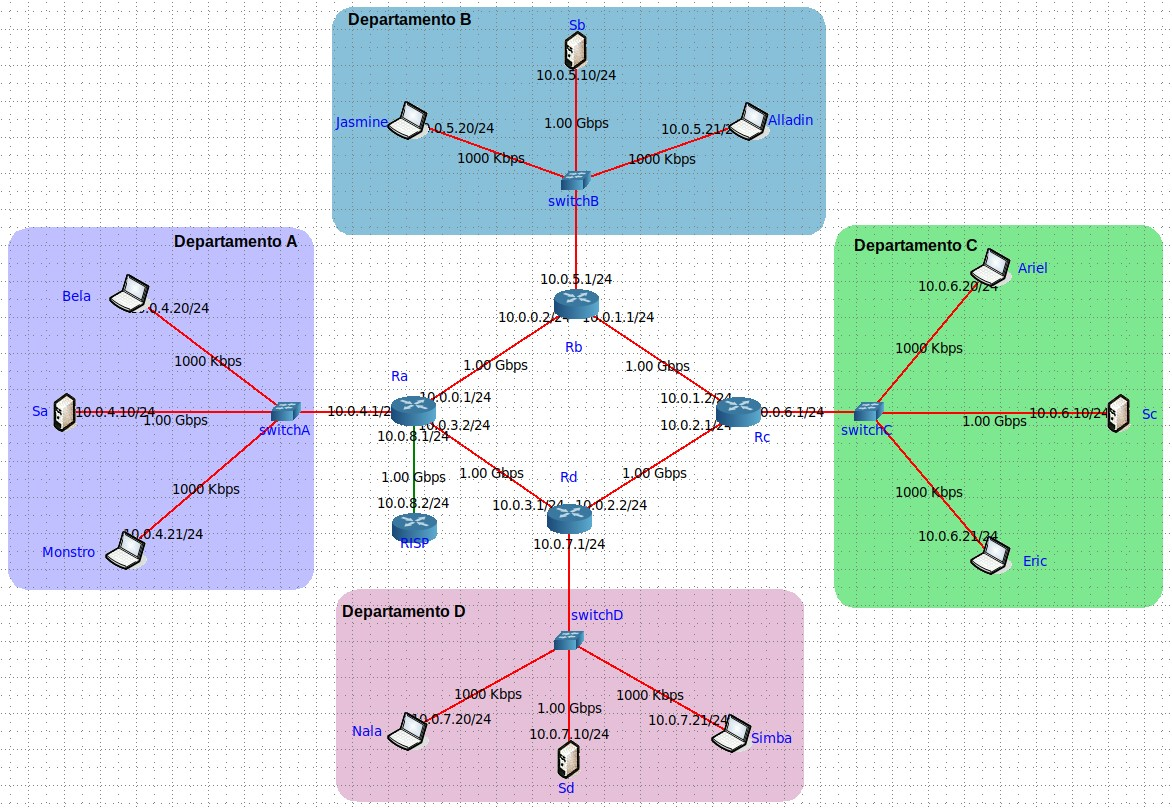
\includegraphics[width=500pt]{images/ParteII/Questao1/TopologiaOriginal.jpg}
    \caption{Topologia LEI-RC.} \label{parteII-questao1-topologia}
    \end{figure}
    
    
    

\subsubsection{Tratam-se de endereços privados? Porquê?}
    
    \par Geralmente os endereços privados encontram-se reservados entre intervalos específicos geridos pela \textit{Internet Assigned Numbers Authority (IANA)} e, por essa razão, não podem ser atribuídos de forma arbitrária. Apresentamos, então, alguns intervalos reservados para endereços privados: 
    
        \begin{itemize}
            \item 10.0.0.0 - 10.255.255.255 / 8
            \item 172.16.0.0 - 172.31.255.255 / 12
            \item 192.168.0.0 - 192.168.255.255 / 16
        \end{itemize}
        
        \par Visto que todos os endereços presentes na topologia se encontram incluídos no intervalo de endereços do primeiro ponto, podemos afirmar que os endereços se tratam de endereços privados.
        
        
        
        
    
\subsubsection{Porque razão não é atribuido um endereço IP aos switches?}

    \par Os \textit{switches} tratam-se de dispositivos que simplesmente conectam todos os elementos da rede. Estes atuam como ponte ou unidade de controlo para que os dispositivos possam comunicar entre si.
    Estes pertencem à camada dois do modelo de referência OSI, ou seja, camada de \textit{Link}. Esta camada está localizada diretamente abaixo da camada de rede (camada três) que funciona sobre endereços IP, no entanto, a camada de \textit{Link} utiliza endereços MAC (endereços físicos) daí não ter sido atribuído endereço IP aos \textit{switches}.  
    
    
    
    
    
\subsubsection{Usando o comando \textit{\textbf{ping}} certifique-se que existe conectividade IP interna a cada departamento (e.g. entre um laptop e o servidor respetivo).}

    \par Como podemos ver pelas figuras apresentadas abaixo, existe conectividade interna nos vários departamentos uma vez que existe resposta (\textit{echo reply}) ao envio de pacotes (\textit{echo request}) entre dispositivos no mesmo departamento.
    
    \begin{minipage}{0.5\linewidth}
    \centering
        \begin{figure}[H]
        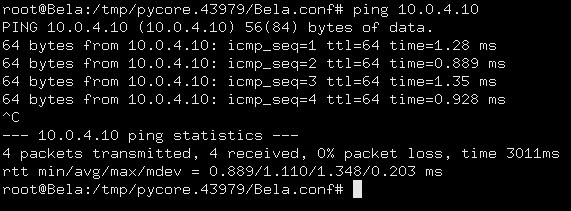
\includegraphics[width=\linewidth]{images/ParteII/Questao1/parteII-questao1-d-Bela.jpg}
        \caption{Departamento A (Bela - Sa).} \label{parteII-questao1-ping-Bela-SA}
        \end{figure}
    \end{minipage}
    \begin{minipage}{0.5\linewidth}
    \centering
        \begin{figure}[H]
        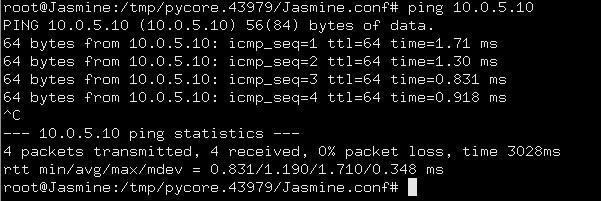
\includegraphics[width=\linewidth]{images/ParteII/Questao1/parteII-questao1-d-Jasmine.jpg}
        \caption{Departamento B (Jasmine -Sb).} \label{parteII-questao1-ping-Jamsmine-SB}
        \end{figure}
    \end{minipage}
    
    \begin{minipage}{0.5\linewidth}
    \centering
         \begin{figure}[H]
        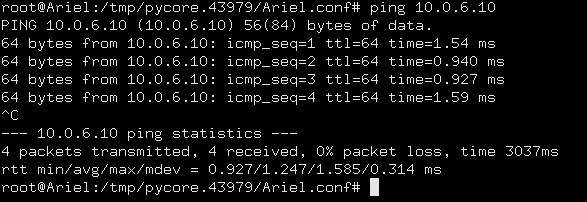
\includegraphics[width=\linewidth]{images/ParteII/Questao1/parteII-questao1-d-Ariel.jpg}
        \caption{Departamento C (Ariel - Sc).} \label{parteII-questao1-ping-Ariel-SC}
        \end{figure}
    \end{minipage}
    \begin{minipage}{0.5\linewidth}
    \centering
        \begin{figure}[H]
        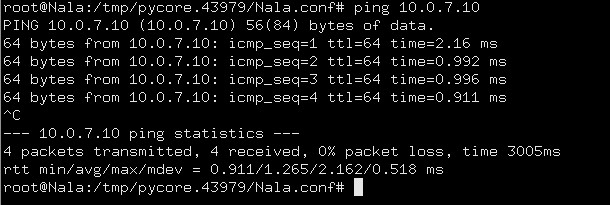
\includegraphics[width=\linewidth]{images/ParteII/Questao1/parteII-questao1-d-Nala.jpg}
        \caption{Departamento D (Nala - Sd).} \label{parteII-questao1-ping-Nala-SD}
        \end{figure}    
    \end{minipage}
    
    
    
    
    
    
\subsubsection{Execute o número mínimo de comandos \textit{\textbf{ping}} que lhe permite verificar a existência de conectividade IP entre departamentos.}

    \par Para verificar a conectividade IP entre os vários departamentos, apenas executamos o comando \textit{ping} duas vezes, sendo estas: 
    
        \begin{itemize}
            \item Departamento A $\xrightarrow[]{}$ Departamento C (Figura \ref{parteII-questao1-ping-A-C})
            
            \item Departamento D $\xrightarrow[]{}$ Departamento B (Figura \ref{parteII-questao1-ping-D-B})
        \end{itemize}
    
    \par Uma vez que o \textit{ping} do departamento A para o C garante que o tráfego na direção horizontal da topologia está a ser encaminhado corretamente e o \textit{ping} do departamento D ao B garante o bom encaminhamento vertical do tráfego da topologia, conseguimos, assim, garantir a conectividade entre todos os departamentos pois temos garantias do correto funcionamento dos quatro \textit{routers}.
    
    \begin{minipage}{0.5\linewidth}
    \centering
        \begin{figure}[H]
        \centering
        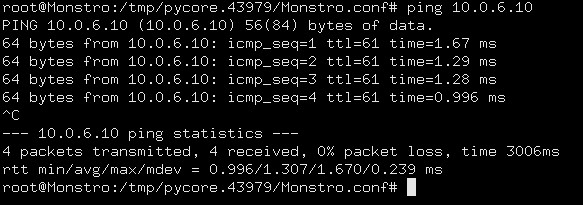
\includegraphics[width=\linewidth]{images/ParteII/Questao1/parteII-questao1-e-A-C.jpg}
        \caption{Ping do Departamento A para o C.} \label{parteII-questao1-ping-A-C}
        \end{figure}
    \end{minipage}
    \begin{minipage}{0.5\linewidth}
    \centering
        \begin{figure}[H]
        \centering
        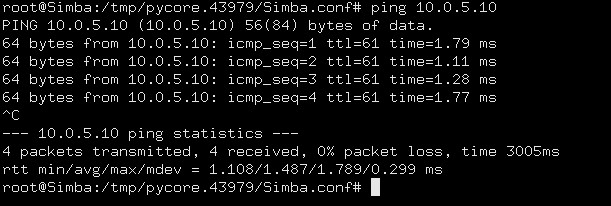
\includegraphics[width=\linewidth]{images/ParteII/Questao1/parteII-questao1-e-D-B.jpg}
        \caption{Ping do Departamento D para o B.} \label{parteII-questao1-ping-D-B}
        \end{figure}
    \end{minipage}
    
    
    
    
\paragraph{}
\subsubsection{Verifique se existe conectividade IP do portátil Bela para o router de acesso Risp.}

    \par Como podemos verificar pela Figura \ref{parteII-questao1-f-BelaISP}, ao executar o comando \textit{ping} do portátil Bela para o \textit{router} de acesso Risp, este obtém resposta provando assim a conectividade entre os mesmos.
    
    \textbf{\begin{figure}[H]
    \centering
    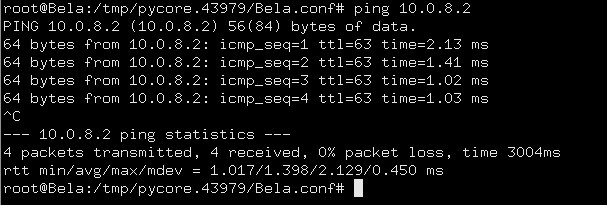
\includegraphics[width=300pt]{images/ParteII/Questao1/parteII-questao1-f-BelaISP.jpg}
    \caption{Ping Bela - Risp} \label{parteII-questao1-f-BelaISP}
    \end{figure}}














\newpage
\subsection{Questão 2 - Tabelas de Encaminhamento (Bela - Ra)}

\subsubsection{Execute o comando \textit{\textbf{netstat -rn}} por forma a poder consultar a tabela de encaminhamento unicast (IPV4). Interprete as várias entradas de cada tabela}
    
    \begin{figure}[H]
    \centering
    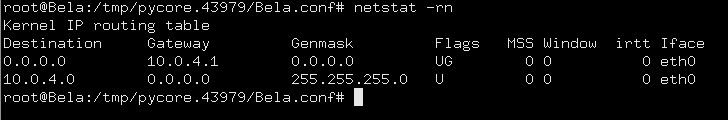
\includegraphics[width=450pt]{images/ParteII/Questao2/parteII-questao2-a-Bela.jpg}
    \caption{Tabela de Encaminhamento do \textit{host} Bela.} \label{parteII-questao2-a-tabelaBela}
    \end{figure} 
    
    \begin{figure}[H]
    \centering
    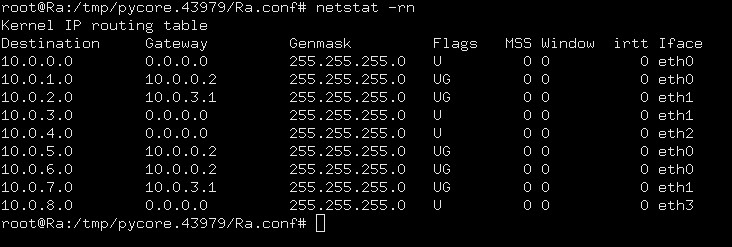
\includegraphics[width=450pt]{images/ParteII/Questao2/parteII-questao2-a-RA.jpg}
    \caption{Tabela de Encaminhamento do \textit{router} Ra.} \label{parteII-questao2-a-tabelaRa}
    \end{figure} 
        
    \par Uma tabela de encaminhamento fornece instruções para determinar o próximo salto de um pacote de dados numa rede IP. Como tal, tem de possuir parâmetros que permitam executar esse mesmo encaminhamento. Assim, apresentamos, também em formato tabela, a descrição das várias colunas da tabela de encaminhamento dos dois dispositivos:
    
    \begin{center}
        \begin{tabular}{|c|c|}
        \hline
            \cline{1-2}
            Coluna & Descrição  \\
            \hline \hline
            Destination & endereço IP de rede destino \\
            Gateway & endereço IP do próximo salto \\
            Genmask & máscara a aplicar à coluna Destination \\
            Flags* & informação sobre a rota \\
            MSS & tamanho máximo de segmentos TCP \\
            Window & tamanho \textit{default} da janela TCP \\
            irtt & RTT estimado (inicial) \\
            Iface & interface de saída \\
            \cline{1-2}
        \end{tabular}
    \end{center}
    
    \par * Existem várias \textit{flags} disponíveis, no entanto, nas figuras acima, apenas percepcionamos a \textbf{U} e \textbf{G}. A presença da \textit{flag} U determina que a rota está disponível e a \textit{flag} G indica a utilização da \textit{Gateway}.
    
    \newpage
    \par Relativamente às entradas das duas tabelas de encaminhamento, estas possuem a informação necessária para os pacotes de dados enviados por estes conseguirem alcançar o seu destino. 
    
    \par Em concreto, o portátil Bela apenas possui duas entradas que por sua vez descrevem a única interface de saída do mesmo, estando a primeira definida como rota por defeito e a segunda como próximo salto caso o destino seja a sua própria rede. Assim, o portátil Bela consegue assegurar o tráfego dos seus pacotes uma vez que, por defeito, redireciona o tráfego para o \textit{router} Ra.
    
    \par O \textit{router} Ra possui entradas para todas as sub-redes presentes na topologia, permitindo assim encaminhar tráfego para as mesmas. Para além disto, conseguimos denotar que todas as entradas com endereço IP 0.0.0.0 na coluna \textit{Gateway} têm como destino uma sub-rede da qual o \textit{router} já faz parte, isto acontece porque uma vez que o \textit{router} já está integrado na sub-rede, então já não existe \textit{gateway}.
    
    
    

\paragraph{}
\subsubsection{Diga, justificando, se está a ser usado encaminhamento estático ou dinâmico}

    \begin{figure}[H]
    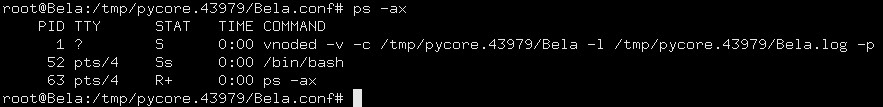
\includegraphics[width=\linewidth]{images/ParteII/Questao2/parteII-questao2-b-Bela.jpg}
    \caption{Resultado do comando no \textit{host} Bela.} \label{parteII-questao2-b-encaminhamentoBela}
    \end{figure} 
    
    \begin{figure}[H]
    \centering
    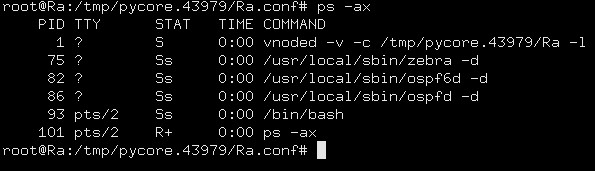
\includegraphics[width=400pt]{images/ParteII/Questao2/parteII-questao2-b-RA.jpg}
    \caption{Resultado do comando no \textit{router} RA.} \label{parteII-questao2-b-encaminhamentoRA}
    \end{figure} 
    
    
    \par Pelas Figuras \ref{parteII-questao2-b-encaminhamentoBela} e \ref{parteII-questao2-b-encaminhamentoRA} conseguimos perceber algumas diferenças nos processos que estão a decorrer em cada um dos dispositivos. A presença de um processo que termina com \textit{\textbf{ospf}} significa que o protocoloo OSPF está a ser utilizado. O protocolo OSPF (\textit{Open Shortest Path First}), é um protocolo de descoberta de vizinhos, isto é, os \textit{routers} ou \textit{hosts} depois de garantirem que as suas interfaces estão funcionais, enviam pacotes '\textit{Hello}' para descobrir os dispositivos adjacentes (vizinhos) e as rotas conhecidas pelos mesmos. A utilização do protocolo OSPF garante um encaminhamento dinâmico, uma vez que este, através da comunicação entre os vários dispositivos, define o melhor caminho.
    Assim, podemos concluir que o portátil Bela não utiliza encaminhamento dinâmico, contrariamente ao \textit{router} Ra que utiliza.
    
    
    
    
    
\subsubsection{Admita que, por questões administrativas, a rota por defeito (\textit{\textbf{0.0.0.0}} ou \textit{\textbf{default}}) deve ser retirada definitivamente da tabela de encaminhamento do servidor Sa. Use o comando \textit{\textbf{route delete}} para o efeito. Que implicações tem esta medida para os utilizadores da LEI-RC que acedem ao servidor. Justifique.}
    
    \paragraph{}
    \paragraph{}
    \begin{figure}[H]
    \centering
    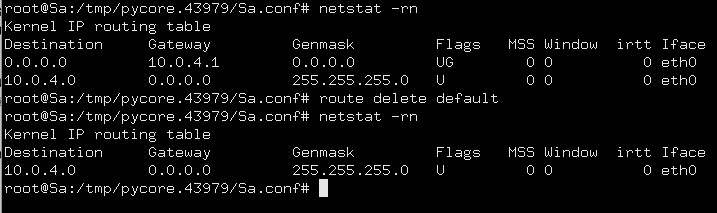
\includegraphics[width=400pt]{images/ParteII/Questao2/parteII-questao2-c-SA-delete.jpg}
    \caption{Comando \textit{route delete} executado.} \label{parteII-questao2-c-deleteSA}
    \end{figure} 
    

    \par Pela Figura \ref{parteII-questao2-c-deleteSA} conseguimos perceber que após retirada da rota por defeito da tabela de encaminhamento do servidor Sa, este apenas possui a entrada para o encaminhamento de dados que tenham como destino a sua própria sub-rede. Em consequência, e sabendo que a rota por defeito é a rota a seguir caso não exista uma entrada específica na tabela de encaminhamento para a rede destino requerida, ao retirarmos esta mesma entrada, estamos a impossibilitar a comunicação do servidor com dispositivos que se encontrem fora da sua sub-rede (10.0.4.0), pois este apesar de conseguir receber dados não irá conseguir responder. Assim, apresentamos de seguida o comando \textit{ping} com origem num \textit{host} de outra sub-rede (servidor Sc), provando que o servidor Sa não consegue comunicar de volta, pois a percentagem de pacotes perdidos (\textit{packet loss}) é de 100\%:
    
    \paragraph{}
    \begin{figure}[H]
    \centering
    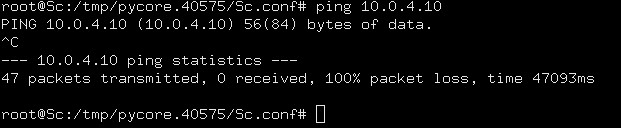
\includegraphics[width=400pt]{images/ParteII/Questao2/questao2-pingSAdeleted.jpg}
    \caption{Comando \textit{ping} ao servidor Sa.} \label{parteII-questao2-Sc-Sa-deleteSA-ping}
    \end{figure} 
    
    
    
\subsubsection{Não volte a repor a rota por defeito. Adicione todas as rotas estáticas necessárias para restaurar a conectividade para o servidor Sa, por forma a contornar a restrição imposta na alínea c). Utilize para o efeito o comando \textit{\textbf{route add}} e registe os comandos que usou.}
    
    \begin{figure}[H]
    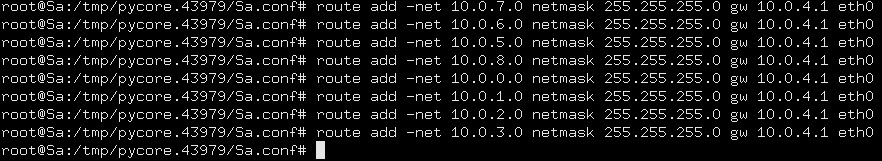
\includegraphics[width=\linewidth]{images/ParteII/Questao2/parteII-questao2-d-SA-ADD.jpg}
    \caption{Comandos utilizados para adicionar as rotas à tabela de encaminhamento.} \label{parteII-questao2-d-novoTabelaSA}
    \end{figure} 
    
    
    \par Como podemos ver pela Figura \ref{parteII-questao2-d-novoTabelaSA}, foram adicionadas estaticamente todas as sub-redes presentes na topologia LEI-RC utilizando como \textit{gateway} o endereço IP do \textit{router} Ra que anteriormente estava definida como rota por defeito, permitindo restaurar a conectividade para o servidor Sa.
    
    
    
    
\paragraph{}
\subsubsection{Teste a nova política de encaminhamento garantindo que o servidor está novamente acessível, utilizando para o efeito o comando \textit{\textbf{ping}}. Registe a nova tabela de encaminhamento do servidor.}
  
    \begin{figure}[H]
    \centering
    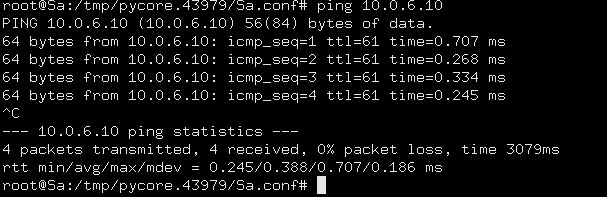
\includegraphics[width=400pt]{images/ParteII/Questao2/parteII-questao2-e-SA-PING.jpg}
    \caption{Comando \textit{ping} do servidor Sa para o servidor Sc.} \label{parteII-questao2-e-PING}
    \end{figure} 
    
    
    \par Pela Figura \ref{parteII-questao2-e-PING}, conseguimos denotar que o servidor está novamente acessível, uma vez que utilizamos o comando \textit{ping} com destino no servidor Sc, estando este presente numa sub-rede diferente da do servidor Sa, provando assim que o servidor consegue novamente comunicar com os dispositivos localizados fora da sua sub-rede. 

    \paragraph{}
    \begin{figure}[H]
    \centering
    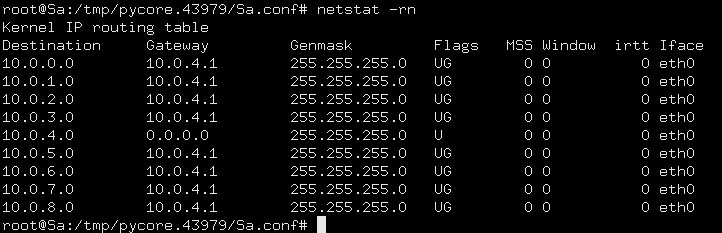
\includegraphics[width=400pt]{images/ParteII/Questao2/parteII-questao2-e-SA-TABELA.jpg}
    \caption{Tabela de Encaminhamento do servidor Sa.} \label{parteII-questao2-e-TABELA}
    \end{figure} 
  
  
    \par De seguida, consultamos a nova tabela de encaminhamento do servidor (Figura \ref{parteII-questao2-e-TABELA}), denotando as entradas que substituíram a rota por defeito, ou seja, entradas de todas as sub-redes da topologia. Adicionalmente, é de notar que a rota por defeito tem como objetivo, entre outros, reduzir a tabela de encaminhamento, agregando todas as rotas que possuem como endereço IP destino sub-redes exteriores, neste caso, ao servidor. Assim, o crescimento da tabela de encaminhamento após retirada da rota por defeito é notório como podemos comprovar pela comparação das Figuras \ref{parteII-questao2-c-deleteSA} (após retirada da rota por defeito) e \ref{parteII-questao2-e-TABELA} (após introdução estática das rotas).
  
  
  
  
  
  
  
  
  
  
  
  
  
\newpage  
\subsection{Questão 3 -  Definição de Sub-redes}

\subsubsection{Considere que dispõe apenas do endereço da rede IP 192.168.XXX.128/25, em que XXX é o decimal correspondendo ao seu número de grupo (PLXXX). Defina um novo esquema de endereçamento para as redes dos departamentos (mantendo as redes de acesso externo e \textit{backbone} inalteradas), sabendo que o número de departamentos pode vir a aumentar no curto prazo. Atribua endereços às interfaces dos vários sistemas envolvidos. Assuma que todos os endereços de sub-redes são usáveis.}

    \par 
    
    \begin{figure}[H]
    \centering
    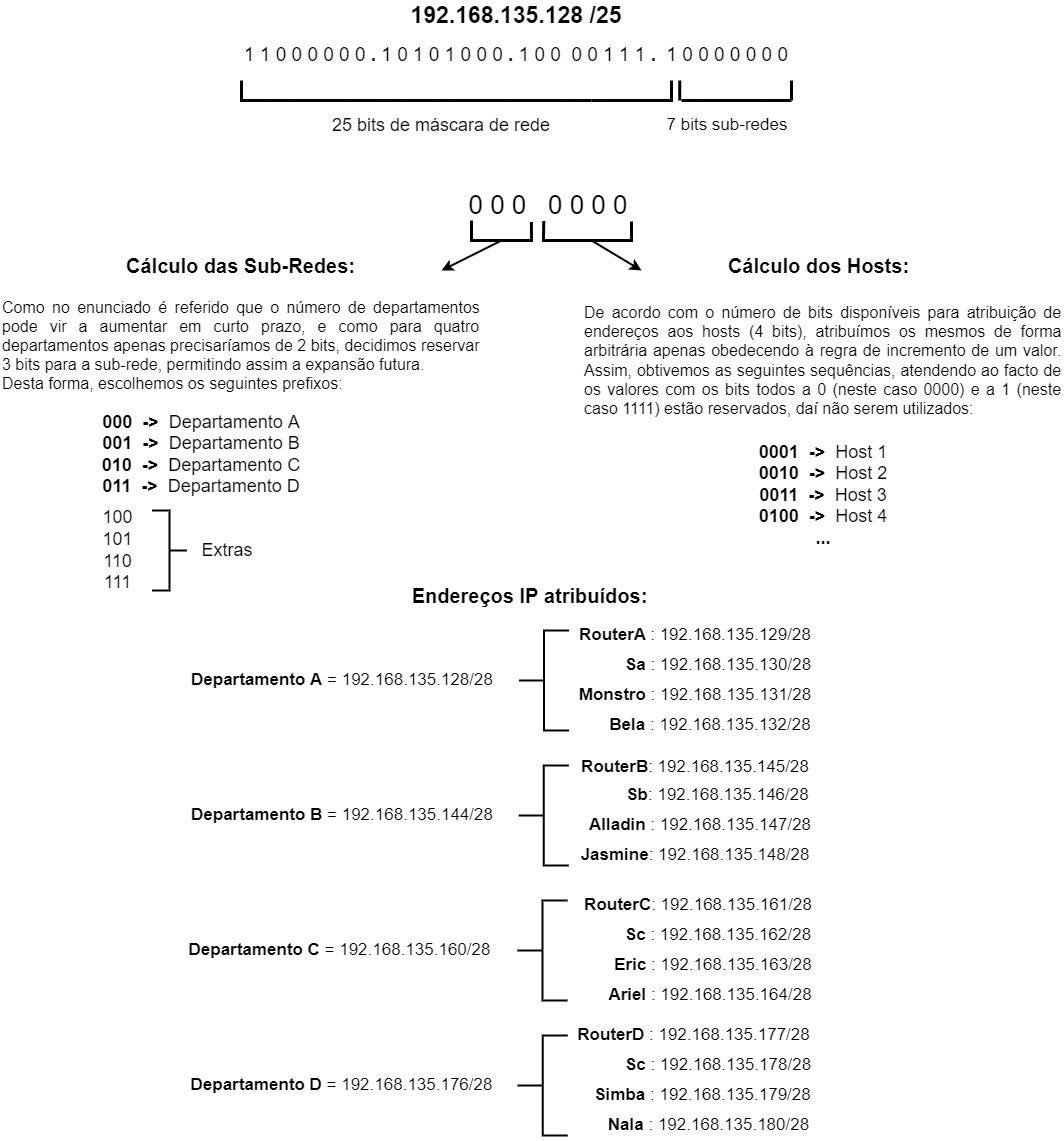
\includegraphics[width=500pt]{images/ParteII/Questao3/Questao3-ParteII-RC-Questao3.drawio.png}
    \label{parteII-questao3-subnetting}
    \end{figure}
    
    \par \textbf{NOTA:} Por simplificação, na figura apresentada de seguida, os endereços IP das interfaces de ligação dos \textit{routers} não estão presentes, mas é subentendida a sua presença. Assim, apresentamos uma vista simplificada da topologia com as diversas sub-redes (Departamentos):
    \paragraph{}
    \begin{figure}[H]
    \centering
    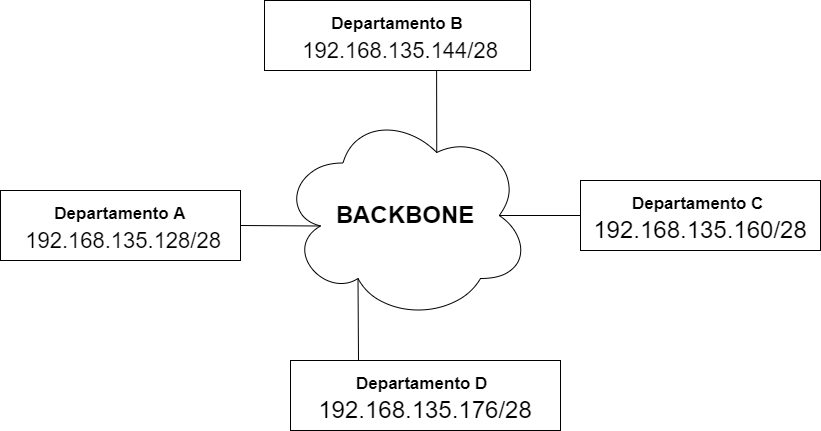
\includegraphics[width=450pt]{images/ParteII/Questao3/Questao3-Topologia.png}
    \caption{Vista simplificada da rede após aplicação de \textit{Subnetting}.}
    \label{parteII-questao3-topologia}
    \end{figure}
    
    %\par Os endereços dos routers ficaram com o primeiro endereço de forma aleatória, podendo estes possuir qualquer valor de endereço no intervalo determinado para a sub-rede.
    
    
    
\paragraph{}    
\subsubsection{Qual a máscara de rede que usou (em formato decimal)? Quantos \textit{hosts} IP pode interligar em cada departamento? Quantos prefixos de sub-rede ficam disponíveis para uso futuro? Justifique.}

    \par A máscara de rede utilizada foi de /28 \textit{bits} (255.255.255.240) uma vez que foram utilizados mais 3 \textit{bits} para representar as diversas sub-redes. Assim, em cada departamento é possível interligar no máximo 14 \textit{hosts} uma vez que todos têm disponíveis para o efeito 4 \textit{bits} (2\textsuperscript{4} - 2). Relativamente aos prefixos de sub-rede disponíveis para uso futuro, sobraram 4 prefixos possíveis, pois, uma vez que foram utilizados 3 \textit{bits} para atribuição de sub-redes, há um total de oito combinações tendo quatro destas sido já atribuídas aos vários departamentos. Assim, sobraram os seguintes prefixos: 100, 101, 110 e 111.
    
    
    

\newpage
\subsubsection{Verifique e garanta que a conectividade IP interna na rede local LEI-RC é mantida. No caso de não existência de conectividade, reveja a atribuição de endereços efetuada e eventuais erros de encaminhamento por forma a realizar as correções necessárias. Explique como procedeu.}

    \paragraph{}
    \paragraph{}
    \begin{figure}[H]
    \centering
    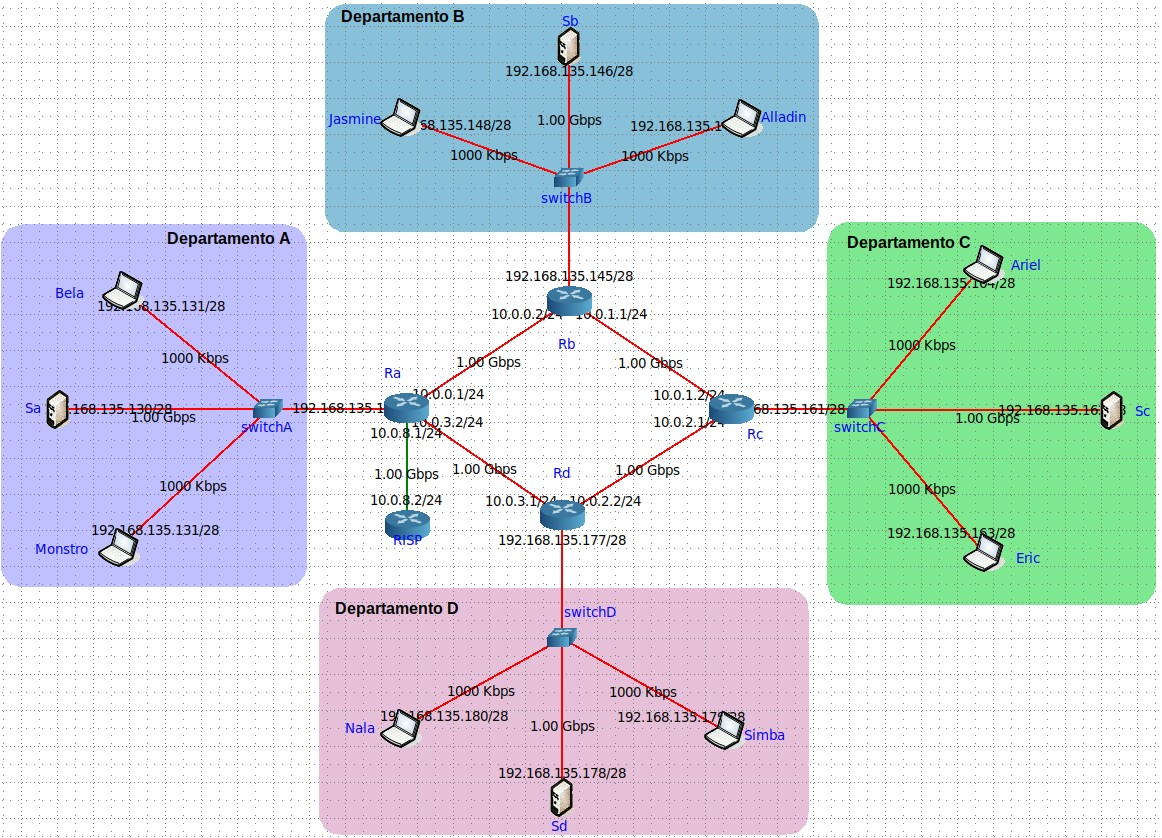
\includegraphics[width=500pt]{images/ParteII/Questao3/TopoSubnetting.jpg}
    \label{parteII-questao3-subnettingNovo}
    \caption{Topologia após aplicação de \textit{Subnetting}.}
    \end{figure}
    
    
    \paragraph{}
    \par Depois da modificação da topologia para a inclusão dos endereços obtidos por \textit{subnetting}, de forma a testar a conectividade na topologia LEI-RC, seguimos o método utilizado na questão 1 da parte II presente neste mesmo relatório, isto é, começamos por verificar a \textbf{conectividade interna} nos vários departamentos, terminando na verificação da \textbf{conectividade inter-departamentos}. Assim, apresentamos a sequência de comandos \textit{ping} utilizados para o efeito:
    
    
    \begin{minipage}{0.5\linewidth}
    \centering
        \begin{figure}[H]
        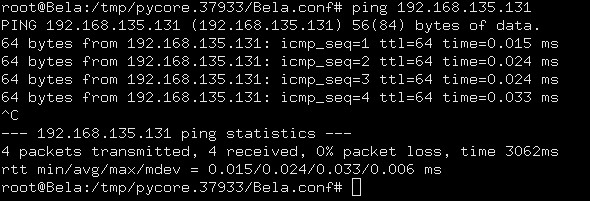
\includegraphics[width=\linewidth]{images/ParteII/Questao3/questao3-DepA-Bela-Monstro.jpg}
        \caption{Departamento A (Bela - Monstro).} \label{parteII-questao3-ping-Bela-Monstro}
        \end{figure}
    \end{minipage}
    \begin{minipage}{0.5\linewidth}
    \centering
        \begin{figure}[H]
        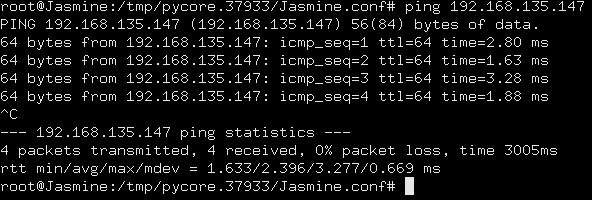
\includegraphics[width=\linewidth]{images/ParteII/Questao3/questao3-DepB-Jasmine-Alladin.jpg}
        \caption{Departamento B (Jasmine - Alladin).} \label{parteII-questao3-ping-Jamsmine-Alladin}
        \end{figure}
    \end{minipage}
    
    \begin{minipage}{0.5\linewidth}
    \centering
         \begin{figure}[H]
        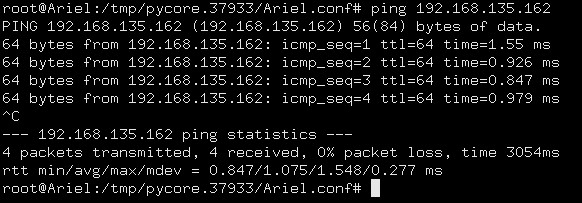
\includegraphics[width=\linewidth]{images/ParteII/Questao3/questao3-DepC-Ariel-Eric.jpg}
        \caption{Departamento C (Ariel - Eric).} \label{parteII-questao3-ping-Ariel-Eric}
        \end{figure}
    \end{minipage}
    \begin{minipage}{0.5\linewidth}
    \centering
        \begin{figure}[H]
        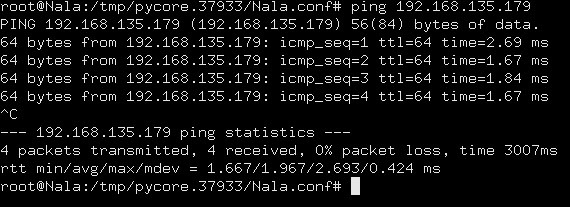
\includegraphics[width=\linewidth]{images/ParteII/Questao3/questao3-DepD-Nala-Simba.jpg}
        \caption{Departamento D (Nala - Simba).} \label{parteII-questao3-ping-Nala-Simba}
        \end{figure}    
    \end{minipage}
    
    
    \paragraph{}
    \begin{minipage}{0.5\linewidth}
    \centering
        \begin{figure}[H]
        \centering
        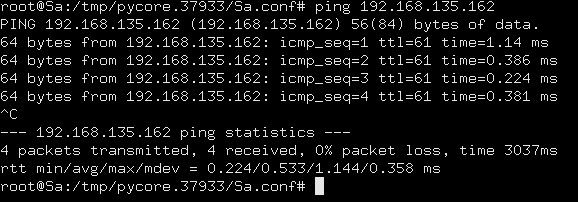
\includegraphics[width=\linewidth]{images/ParteII/Questao3/questao3-DepA-DepC-Sa-Sc.jpg}
        \caption{Ping do Departamento A para o C.} \label{parteII-questao3-ping-A-C}
        \end{figure}
    \end{minipage}
    \begin{minipage}{0.5\linewidth}
    \centering
        \begin{figure}[H]
        \centering
        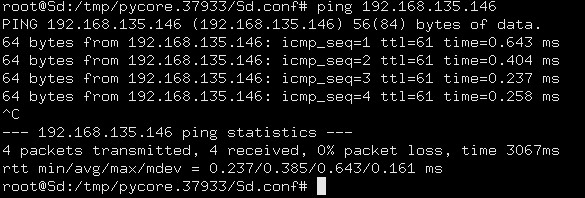
\includegraphics[width=\linewidth]{images/ParteII/Questao3/questao3-Depd-DepB-Sd-Sb.jpg}
        \caption{Ping do Departamento D para o B.} \label{parteII-questao3-ping-D-B}
        \end{figure}
    \end{minipage}